\documentclass[aspectratio=169,10pt]{beamer}
\usetheme{Madrid}
\usecolortheme{default}
\usepackage{graphicx,amsmath,booktabs}
\usepackage[T1]{fontenc}
\definecolor{ink}{HTML}{10304A}
\definecolor{accent}{HTML}{117C83}
\definecolor{gold}{HTML}{D99232}
\definecolor{lightbg}{HTML}{EEF4F6}
\setbeamercolor{structure}{fg=accent}
\setbeamercolor{frametitle}{bg=ink,fg=white}
\setbeamercolor{title}{fg=white,bg=ink}
\setbeamercolor{subtitle}{fg=white}
\setbeamercolor{author}{fg=ink}
\setbeamercolor{block title}{bg=accent,fg=white}
\setbeamercolor{block body}{bg=lightbg,fg=ink}
\setbeamercolor{palette primary}{bg=ink,fg=white}
\setbeamercolor{palette secondary}{bg=accent,fg=white}
\setbeamercolor{palette tertiary}{bg=ink,fg=white}
\setbeamertemplate{navigation symbols}{}
\setbeamertemplate{footline}{\leavevmode\hbox{\begin{beamercolorbox}[wd=.82\paperwidth,ht=2.5ex,dp=1ex,leftskip=1em]{palette primary}\scriptsize Sionna RT for ISAC-based sensing\end{beamercolorbox}\begin{beamercolorbox}[wd=.18\paperwidth,ht=2.5ex,dp=1ex,center]{palette secondary}\scriptsize\insertframenumber{} / \inserttotalframenumber\end{beamercolorbox}}}
\graphicspath{{presentation_assets/}{outputs/mobility_20261104_235027/figures/}{outputs/mobility_20261104_235027/scene_frames/}}
\title[Investigation of Sionna RT]{Investigation of Sionna RT for\\Ray-Traced ISAC-Based Sensing}
\subtitle{Design project presentation}
\author{Nandish Chauhan \quad | \quad Aahan Poddar}
\institute{Indian Institute of Information Technology Vadodara\\[4pt]\small Under the guidance of Dr. Bhupendra Kumar}
\date{}
\begin{document}

\begin{frame}[plain]
\titlepage
\end{frame}

\begin{frame}{Why study radio propagation?}
\begin{columns}[T,onlytextwidth]
\column{.57\textwidth}
\begin{itemize}\setlength\itemsep{10pt}
\item A transmitted signal reaches the receiver through multiple paths.
\item Buildings and surfaces create reflections, diffraction, and blockage.
\item These paths affect communication quality and carry information about the environment.
\end{itemize}
\column{.4\textwidth}
\begin{block}{Key question}
Can a ray tracer generate useful, interpretable path data for communication analysis and future sensing studies?
\end{block}
\end{columns}
\end{frame}

\begin{frame}{ISAC and the scope of this project}
\begin{columns}[T,onlytextwidth]
\column{.48\textwidth}
\begin{block}{ISAC motivation}
Integrated sensing and communication seeks to use radio signals and resources for both connectivity and sensing.
\end{block}
\column{.48\textwidth}
\begin{block}{What we completed}
A moving-receiver ray-tracing simulation and analysis of path geometry, power, delay, and Doppler.
\end{block}
\end{columns}
\vspace{9pt}
\textbf{Project boundary:} No target detector, sensing waveform, range--Doppler processor, or sensing accuracy evaluation has been implemented. These are future uses of the outputs.
\end{frame}

\begin{frame}{End-to-end project workflow}
\begin{enumerate}\setlength\itemsep{8pt}
\item Load the 3D scene and configure materials, antennas, and frequency.
\item Define the receiver's waypoint route and sample its positions.
\item Compute a static radio map and trace paths at each snapshot.
\item Extract complex coefficients, delay, Doppler, angles, and interactions.
\item Calculate channel metrics and export datasets and visualizations.
\end{enumerate}
\vspace{4pt}\begin{block}{Main implementation}
\texttt{mobility\_channel\_study.ipynb} using Sionna RT 2.1.0.
\end{block}
\end{frame}

\begin{frame}{3D scene and modeled environment}
\begin{columns}[c,onlytextwidth]
\column{.54\textwidth}
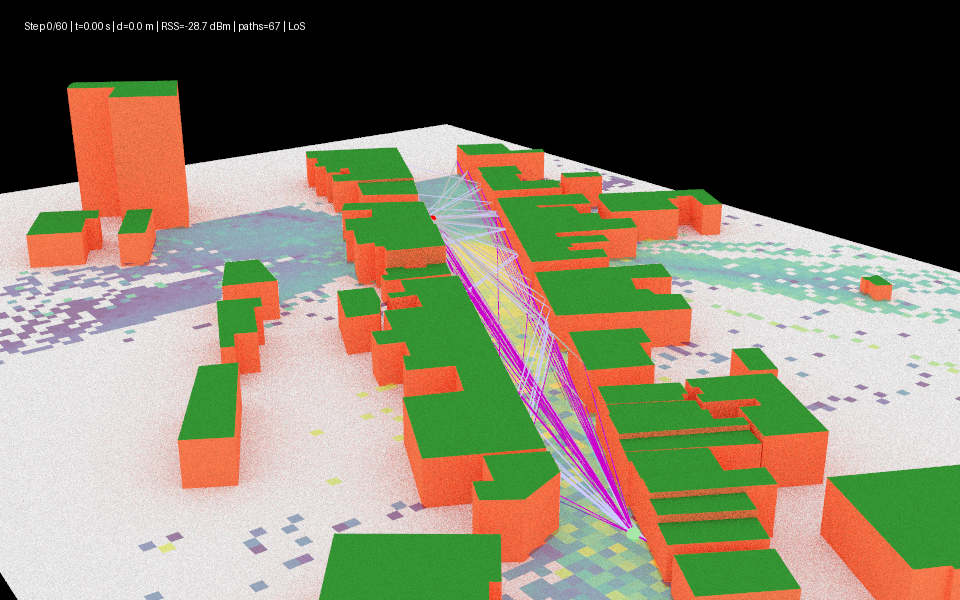
\includegraphics[width=\linewidth]{frame_0000.png}
\column{.44\textwidth}
\begin{itemize}\setlength\itemsep{7pt}
\item Imported scene: building meshes and ground plane.
\item Materials: ITU-style marble, metal, and concrete.
\item Fixed transmitter; receiver travels through the scene.
\item Colored lines show traced paths; the overlay shows the static radio map.
\end{itemize}
\end{columns}
\end{frame}

\begin{frame}{Simulation configuration}
\begin{columns}[T,onlytextwidth]
\column{.56\textwidth}
\small
\begin{tabular}{@{}ll@{}}\toprule
\textbf{Parameter} & \textbf{Saved run}\\\midrule
Frequency / bandwidth & 3.5 GHz / 20 MHz\\
Transmitter power & 44 dBm\\
TX / RX arrays & $4\times4$ / $1\times1$\\
TX position & $(-107,43,10)$ m\\
Receiver height / nominal speed & 2 m / 10 m/s\\
Route / snapshots & 1183.45 m / 61\\
Path depth / samples & 3 / 100,000\\
Radio map & 400 m $\times$ 400 m; 4 m cells\\\bottomrule
\end{tabular}
\column{.41\textwidth}
\begin{block}{Balanced profile}
A practical exploratory configuration; not a convergence or field-validation study.
\end{block}
\vspace{3pt}\small Run: \texttt{mobility\_20261104\_235027}
\end{columns}
\end{frame}

\begin{frame}{What propagation paths are modeled?}
\begin{columns}[T,onlytextwidth]
\column{.5\textwidth}
\begin{itemize}\setlength\itemsep{8pt}
\item \textbf{LoS:} direct path between transmitter and receiver.
\item \textbf{Specular reflection:} path reflected from a surface.
\item \textbf{Refraction:} transmission through a modeled material.
\end{itemize}
\column{.47\textwidth}
\begin{itemize}\setlength\itemsep{8pt}
\item \textbf{Diffraction:} path involving an edge or obstruction.
\item \textbf{Mixed:} a path contains multiple interaction types.
\item Diffuse reflection is enabled, but scattering coefficients are zero; no diffuse-category records appear.
\end{itemize}
\end{columns}
\end{frame}

\begin{frame}[fragile]{How the notebook performs ray tracing}
\begin{columns}[T,onlytextwidth]
\column{.55\textwidth}
\begin{block}{Core sequence (simplified)}
\footnotesize\begin{verbatim}
scene = load_scene(SCENE_PATH)
scene.frequency = 3.5e9
scene.add(tx); scene.add(rx)

for step in range(num_steps):
    rx.position = trajectory[step]
    rx.velocity = velocity[step]
    paths = path_solver(scene, ...)
    a, tau = paths.cir(
        normalize_delays=False,
        out_type="numpy")
\end{verbatim}
\end{block}
\column{.42\textwidth}
\begin{itemize}\setlength\itemsep{7pt}
\item Receiver position and velocity change at each snapshot.
\item The solver retraces valid paths for that position.
\item Channel impulse response data and path metadata are stored.
\item Radio map is computed separately.
\end{itemize}
\end{columns}
\end{frame}

\begin{frame}{Receiver route and radio map}
\begin{columns}[c,onlytextwidth]
\column{.52\textwidth}
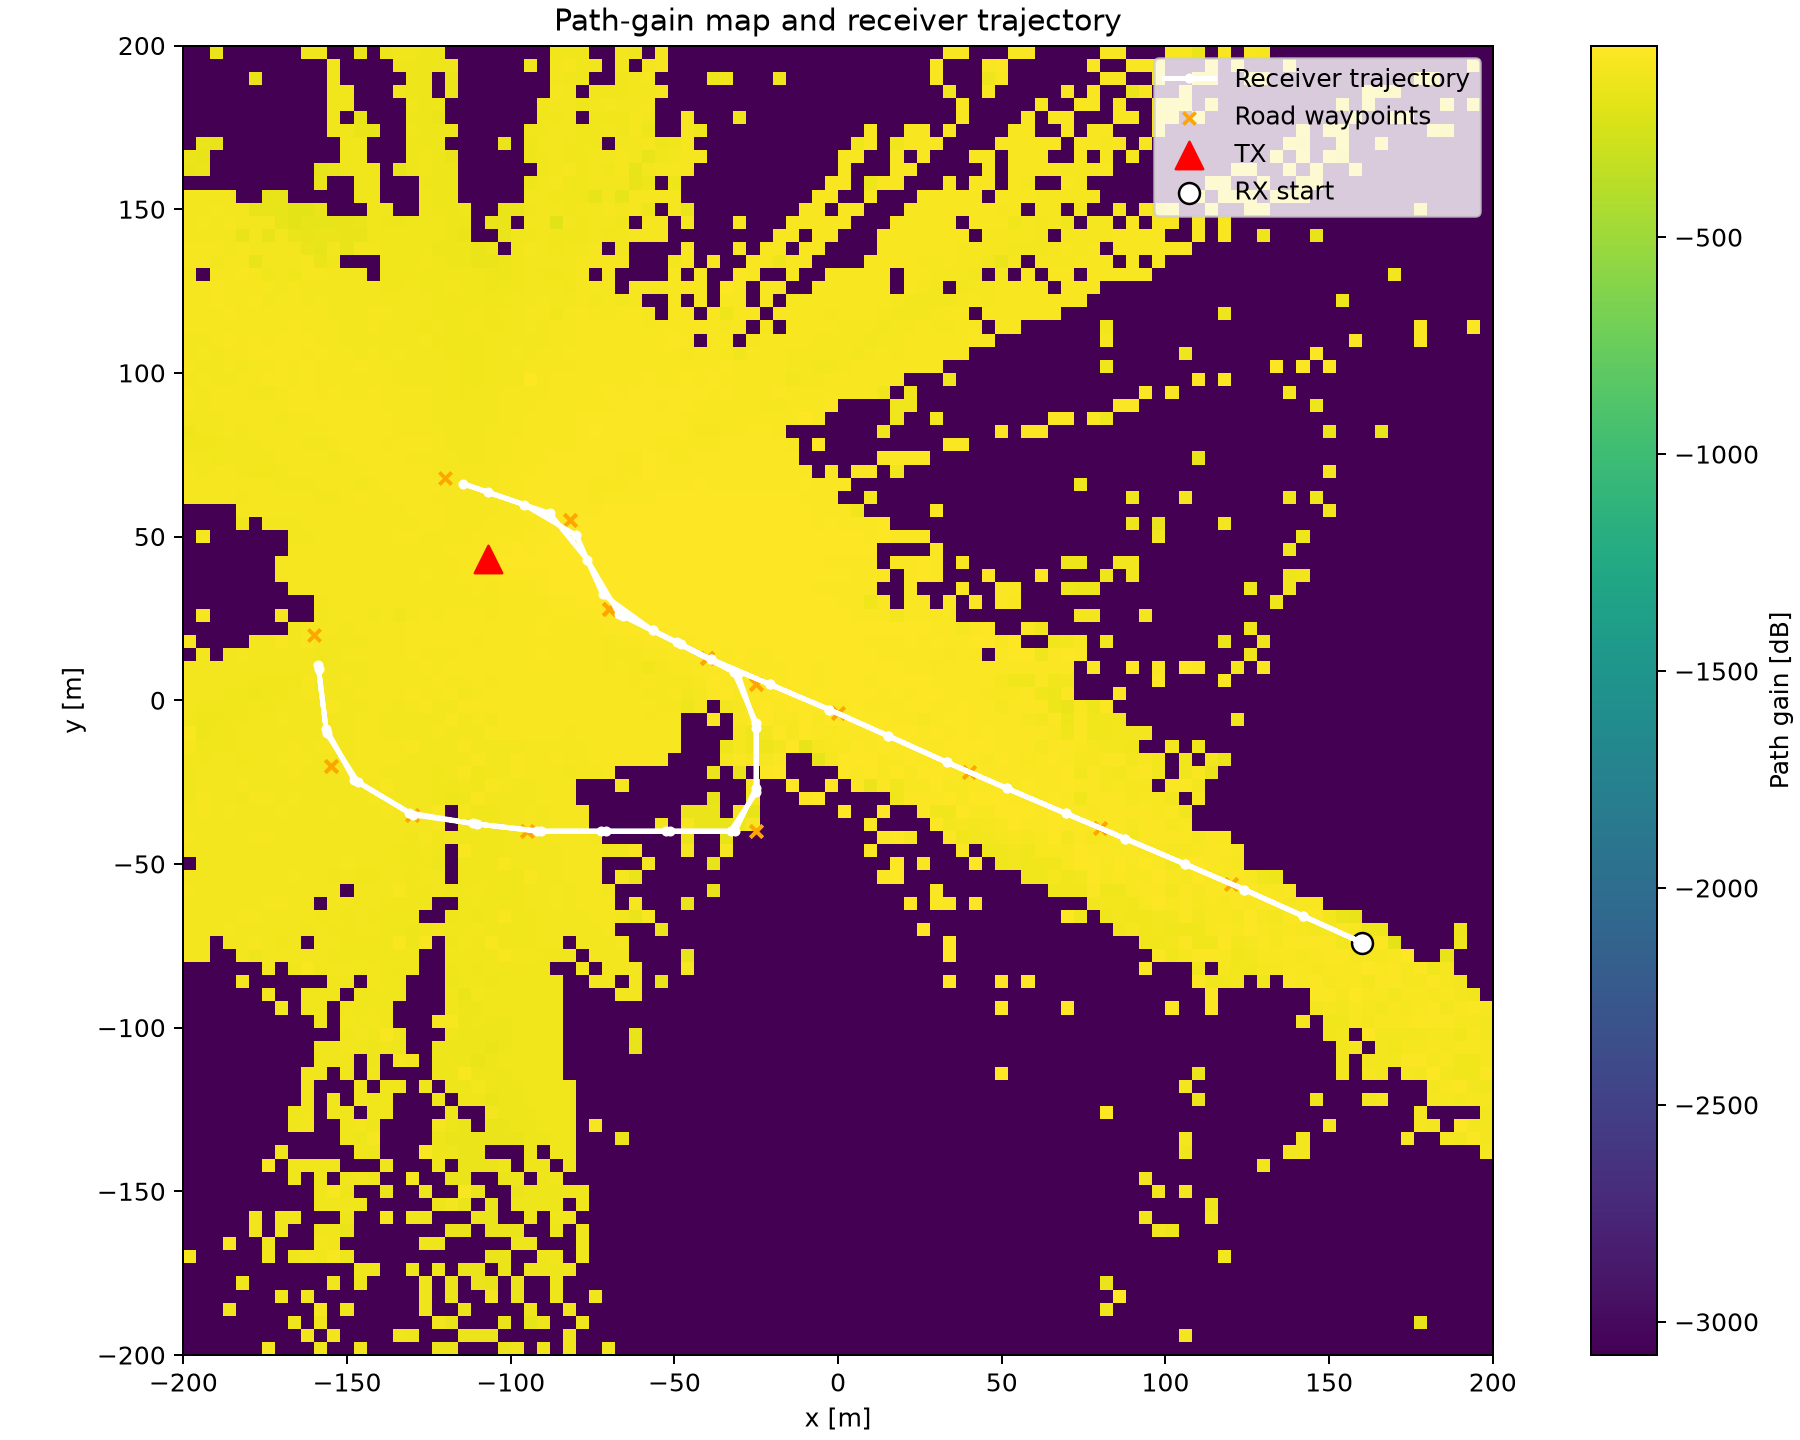
\includegraphics[width=\linewidth]{coverage_and_trajectory.png}
\column{.46\textwidth}
\begin{itemize}\setlength\itemsep{8pt}
\item Waypoints describe an out-and-back route with side-road branches.
\item Route length: \textbf{1183.45 m}; duration: \textbf{118.35 s} at nominal speed.
\item 61 sampled positions; approximately 19.72 m apart along the route.
\item Map height is 1.5 m; receiver height is 2 m. Map gain is not the same quantity as snapshot RSS.
\end{itemize}
\end{columns}
\end{frame}

\begin{frame}{From traced paths to channel metrics}
For each path, equal-weight transmitter-array combining gives an effective complex coefficient $h_i$.
\vspace{6pt}
\begin{columns}[T,onlytextwidth]
\column{.48\textwidth}
\begin{block}{Coherent received power}
\[P_{\rm coh}=P_t\left|\sum_i h_i\right|^2\]
Includes constructive and destructive interference.
\end{block}
\column{.48\textwidth}
\begin{block}{Incoherent path-power sum}
\[P_{\rm inc}=P_t\sum_i |h_i|^2\]
Adds path powers without inter-path phase interference.
\end{block}
\end{columns}
\vspace{5pt}The notebook also calculates power-weighted RMS delay and Doppler spreads, path counts, and thermal-noise-only SNR.
\end{frame}

\begin{frame}{Received power along the route}
\begin{columns}[c,onlytextwidth]
\column{.67\textwidth}
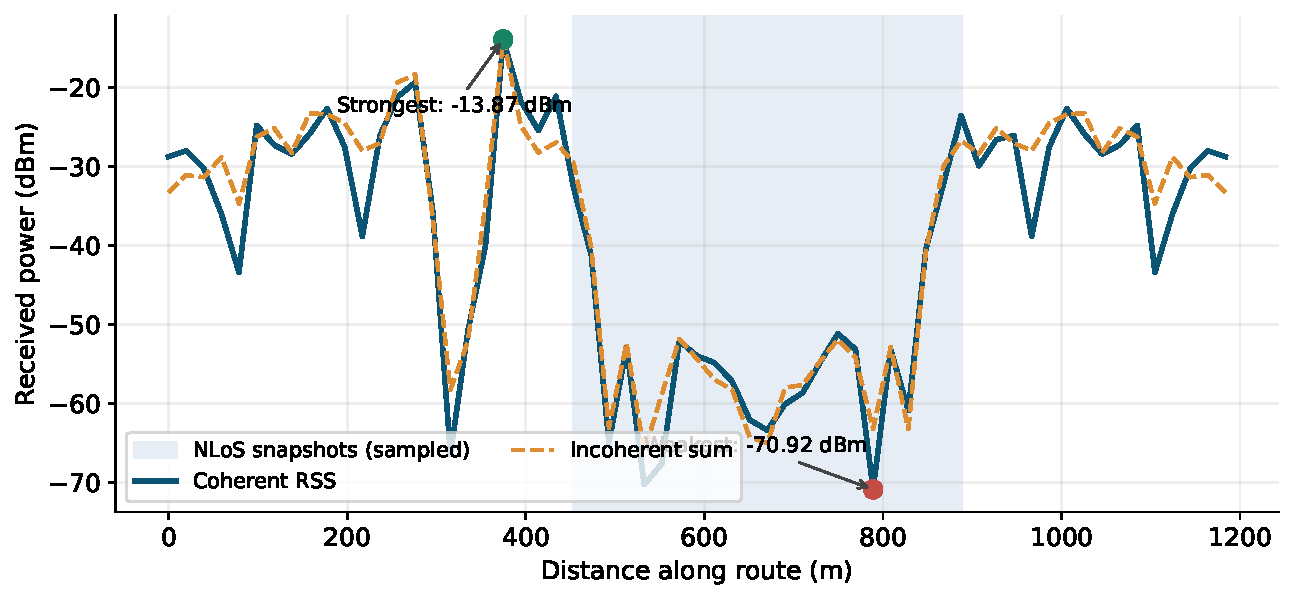
\includegraphics[width=\linewidth]{received_power.pdf}
\column{.31\textwidth}
\begin{itemize}\setlength\itemsep{8pt}
\item Strongest: \textbf{$-13.87$ dBm}, step 19.
\item Weakest: \textbf{$-70.92$ dBm}, step 40.
\item Coherent and incoherent curves differ because of path phase.
\item Shading marks sampled NLoS positions, not exact blockage boundaries.
\end{itemize}
\end{columns}
\end{frame}

\begin{frame}{LoS blockage and reappearance}
\begin{columns}[c,onlytextwidth]
\column{.5\textwidth}
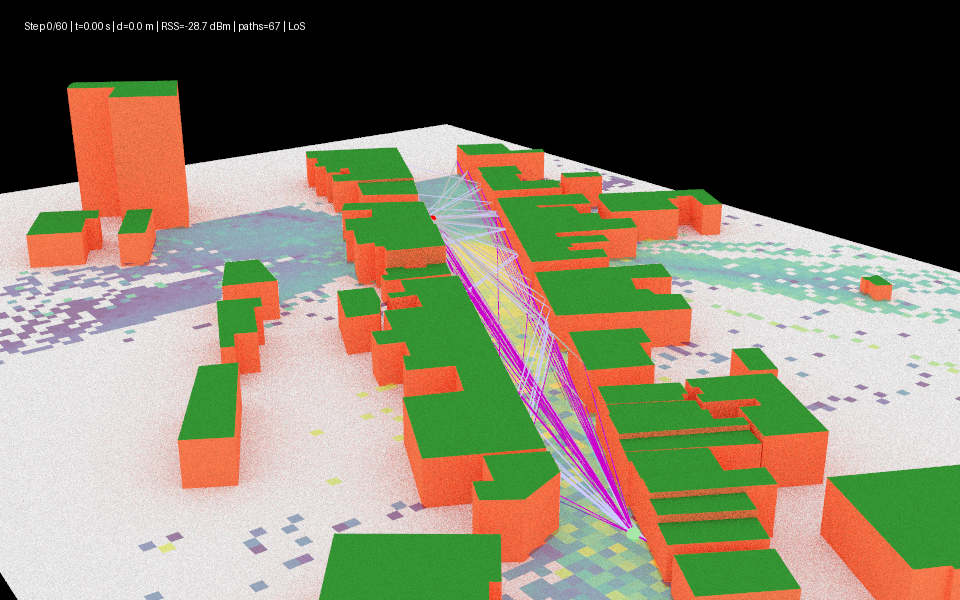
\includegraphics[width=\linewidth]{frame_0000.png}\\[-2pt]
\centering\scriptsize Step 0: LoS, 67 valid paths
\column{.5\textwidth}
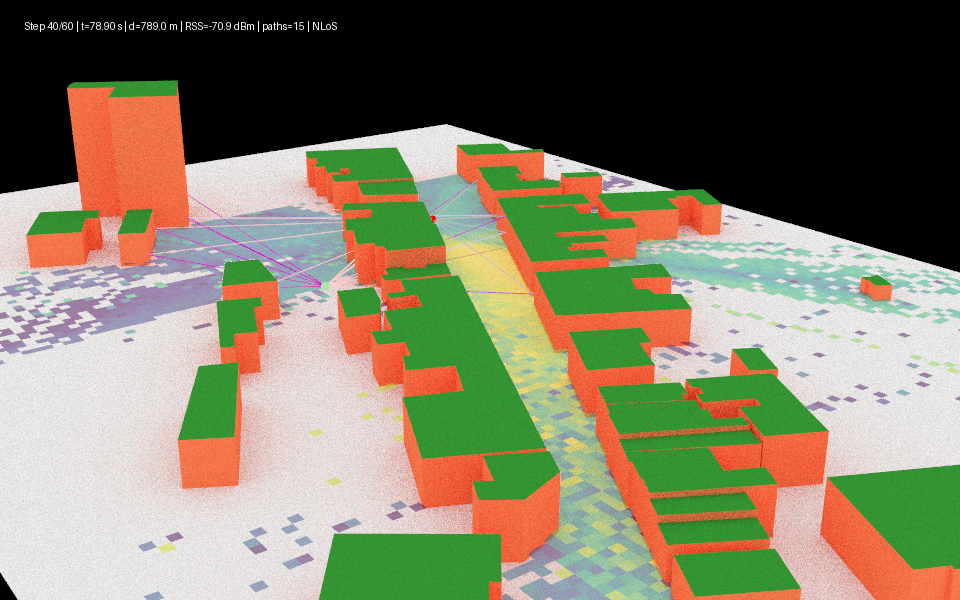
\includegraphics[width=\linewidth]{frame_0020.png}\\[-2pt]
\centering\scriptsize Step 40: NLoS, 15 valid paths
\end{columns}
\vspace{7pt}
\begin{itemize}\setlength\itemsep{3pt}
\item \textbf{39 LoS} and \textbf{22 NLoS} snapshots; LoS is absent at steps 23--44.
\item All 61 snapshots have at least one valid traced path. NLoS is not automatically a service outage.
\end{itemize}
\end{frame}

\begin{frame}{Path delays and propagation mechanisms}
\begin{columns}[c,onlytextwidth]
\column{.55\textwidth}
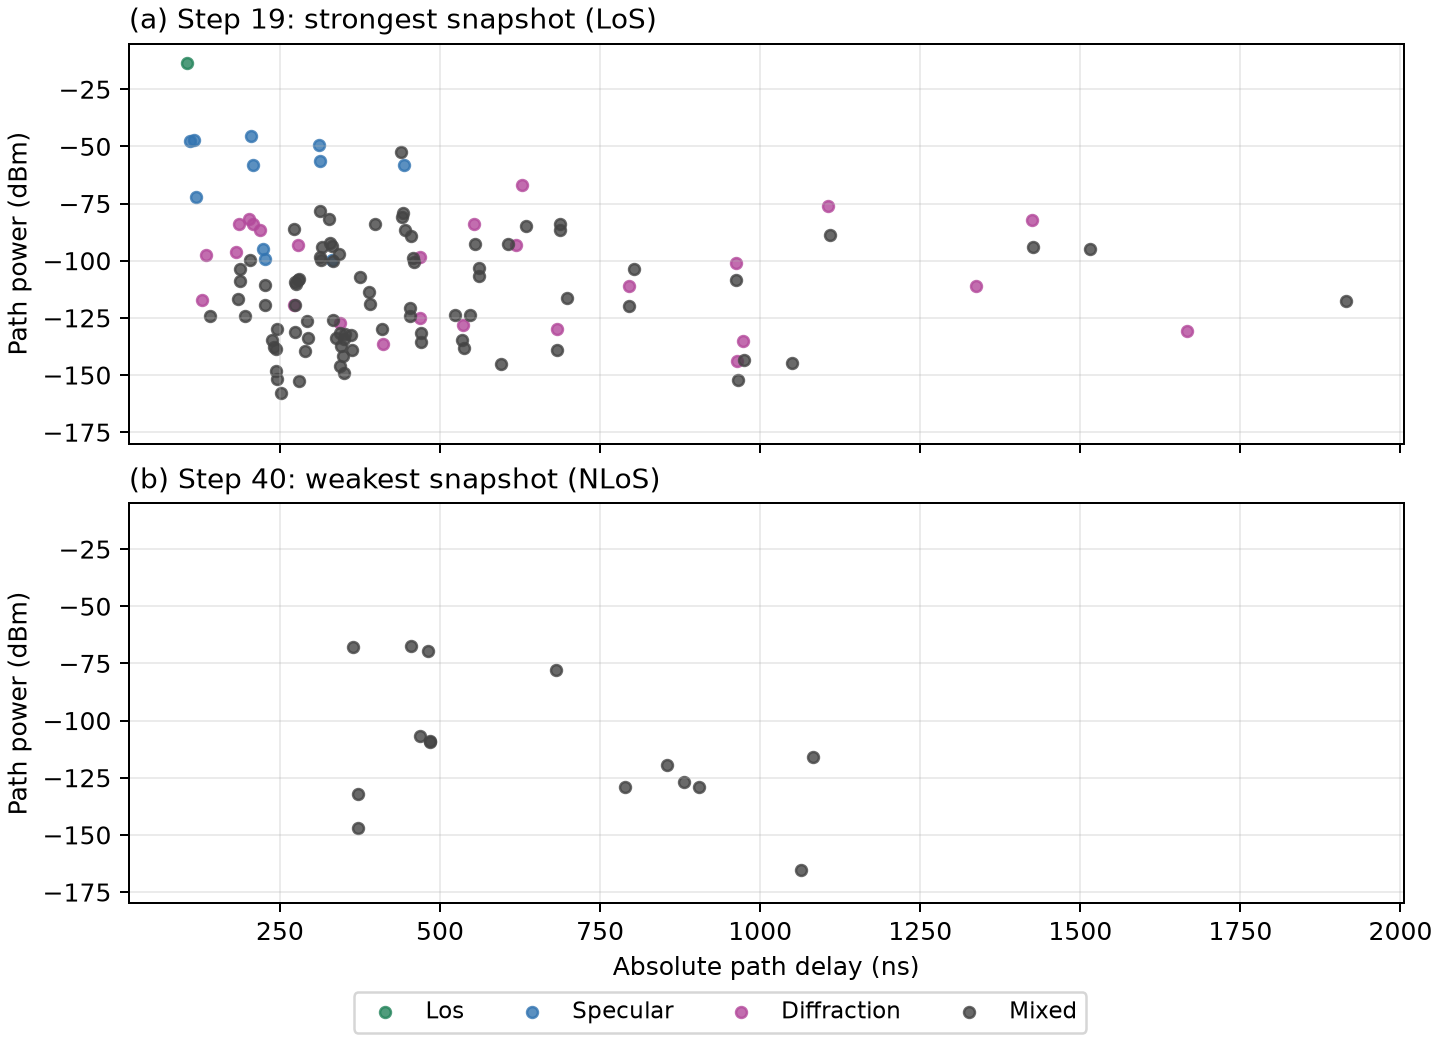
\includegraphics[width=\linewidth]{strong_weak_path_delays.png}
\column{.43\textwidth}
\begin{itemize}\setlength\itemsep{6pt}
\item \textbf{4,826} valid path records across the run.
\item Mixed: 3,426; diffraction-only: 1,010; specular-only: 337.
\item LoS: 39; refraction-only: 14; diffuse-only: 0.
\item Each point is one path's power and absolute delay.
\item Counts do not represent power shares.
\end{itemize}
\end{columns}
\end{frame}

\begin{frame}{Delay and Doppler spread}
\begin{columns}[c,onlytextwidth]
\column{.63\textwidth}
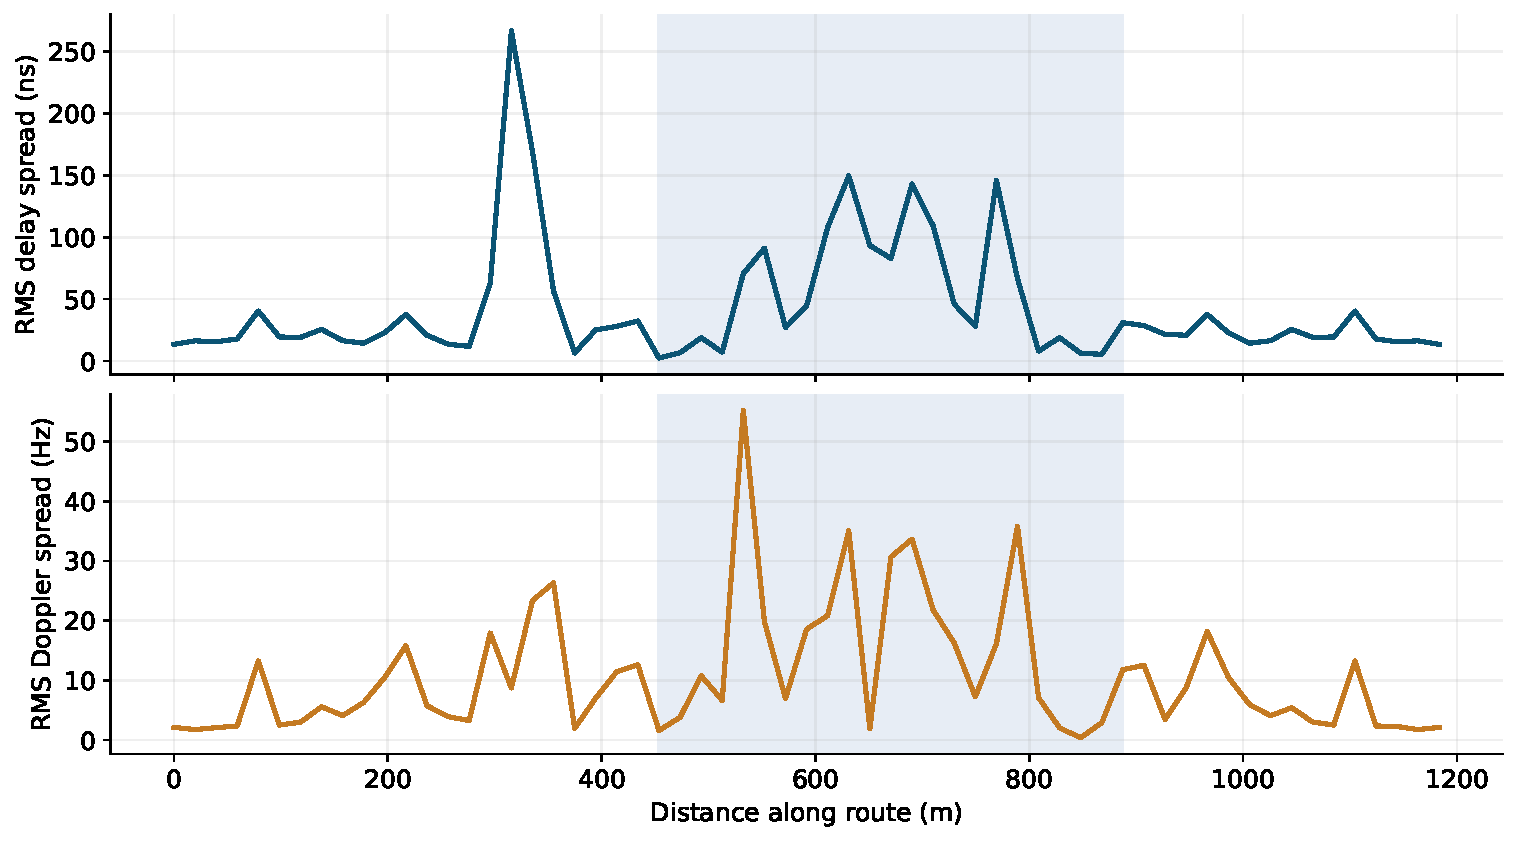
\includegraphics[width=\linewidth]{spread_metrics.pdf}
\column{.35\textwidth}
\begin{itemize}\setlength\itemsep{8pt}
\item RMS delay spread: \textbf{2.40--266.86 ns}.
\item RMS Doppler spread: \textbf{0.39--55.21 Hz}.
\item Values are power-weighted across traced paths.
\item Doppler depends on the velocity used by the snapshot model.
\end{itemize}
\end{columns}
\end{frame}

\begin{frame}{What does the code export?}
\begin{columns}[T,onlytextwidth]
\column{.53\textwidth}
\begin{block}{Numerical data}
\small
\texttt{path\_data.csv}: one record per path.\\[5pt]
\texttt{snapshot\_summary.csv}: aggregate metrics.\\[5pt]
\texttt{channel\_arrays.npz}: numerical channel arrays and validity mask.\\[5pt]
\texttt{run\_config.json}: saved run settings and material audit.
\end{block}
\column{.44\textwidth}
\begin{block}{Visual outputs}
Radio map and trajectory; channel metrics; path geometry; power--delay profile; scene animation.
\end{block}
\vspace{4pt}\small Fields include delay, Doppler, angles, complex coefficient, interaction type, material, and vertices.
\end{columns}
\end{frame}

\begin{frame}{How could these outputs support ISAC?}
\begin{itemize}\setlength\itemsep{9pt}
\item \textbf{Delay:} build channel impulse responses and study path separability.
\item \textbf{Doppler:} investigate signatures related to modeled relative motion.
\item \textbf{Angles and vertices:} relate multipath components to scene geometry.
\item \textbf{Complex coefficients:} create frequency-selective channels for downstream communication or sensing experiments.
\end{itemize}
\vspace{5pt}
\begin{alertblock}{Important distinction}
These are one-way transmitter--receiver paths. They are not automatically radar target ranges; target geometry, a waveform, processing, and validation must be added.
\end{alertblock}
\end{frame}

\begin{frame}{Limitations and next steps}
\begin{columns}[T,onlytextwidth]
\column{.48\textwidth}
\begin{block}{Current limitations}
\begin{itemize}\setlength\itemsep{5pt}
\item One simulated route and static scene; no field measurements.
\item Material properties are not calibrated.
\item No moving targets, interference, or receiver noise figure.
\item Chord-based velocity can underestimate speed near sharp turns.
\end{itemize}
\end{block}
\column{.48\textwidth}
\begin{block}{Next steps}
\begin{itemize}\setlength\itemsep{5pt}
\item Test sensitivity to path samples, depth, and snapshot spacing.
\item Refine trajectory and calibrate materials.
\item Add a defined sensing target and waveform.
\item Implement and validate range, Doppler, or angle estimation.
\end{itemize}
\end{block}
\end{columns}
\end{frame}

\begin{frame}{Conclusion and references}
\begin{block}{Takeaway}
Sionna RT provides interpretable, geometry-based channel data. Our project demonstrates the ray-tracing and analysis pipeline that can serve as a foundation for later ISAC sensing studies.
\end{block}
\vspace{6pt}\small
\textbf{References}\\[3pt]
F. A\"it Aoudia \emph{et al.}, ``Sionna RT: Technical Report,'' arXiv:2504.21719, 2025.\\[3pt]
F. Liu \emph{et al.}, ``Integrated sensing and communications: Toward dual-functional wireless networks for 6G and beyond,'' \emph{IEEE JSAC}, 2022.\\[8pt]
\centering\large\textcolor{accent}{\textbf{Thank you --- Questions?}}
\end{frame}
\end{document}
